
\section{Curves on Toric Surfaces}


\subsection{Introduction}

In this section, we are motivated by the following basic question: given a smooth complete curve $C$ and a toric surface $S$, when does there exist a closed immersion $C \embed S$? Likewise for the smooth complete curve $C$, does there exist some toric surface $S$ which admits a closed immersion $C \embed S$? These questions may be motivated by the toric construction of regular normal crossings models of a curve described by \cite{tim} which requires the curve and various modifications of it to admit embeddings and smooth compactifications in specific toric surfaces. In general, the answer to both questions will be negative. However, for curves which do admit such a toric embedding, we get a strong theory relating the possible toric embeddings to numerical invariants of the curve $C$ as an extension of the well-known numerical constrains on the genus of plane curves. As a first step to understanding embeddings $C \embed S$, notice there are two cases, either $C$ intersects the torus $\Gm{k}^2 \embed S$ or the image of $C$ in $S$ is contained in the toric divisor $D_{\Toric} = \bigcup C_i$ which is a union of curves which are toric varieties. In the later case, since the curve $C$ is irreducible, such an embedding gives an isomorphism between $C$ and an irreducible component of the toric divisor $C_i$ but toric varieties are clearly rational so this case can only occur when $C$ is rational. We will generally ignore this possibility since $\P^1_k$ is the unique smooth complete rational curve. Therefore, we get a trivial positive answer for rational curves since $\P^1_k$ is the unique one dimensional toric variety so $\P^1_k$ can always be embedded in the toric divisor of any toric surface.
\bigskip\\
Thus, when $C$ is non-rational, any embedding $C \embed S$ into a toric surface $S$ must intersect the torus $\Gm{k}^2 \subset S$ giving a closed immersion $U \embed \Gm{k}^2$ of some open affine $U \subset C$. Therefore, our first task will be to understand closed immersions of affine curves $U \embed \Gm{k}^2$.

\begin{lemma}
Every geometrically reduced curve over $k$ is birational to some $U_f \embed \Gm{k}^2$.
\end{lemma}

\begin{proof}
Let $C$ be a curve over $k$. Then $\dim{C} = \trdeg{k}{K(C)}$ by Noetherian normalization so there is a transcendental $t \in K(C)$ such that $K(C)$ is finite over $k(t)$. If we assume that $K(C)  / k(t)$ is separable then by the primitive element theorem $K(C) = k(t)[x]/(m(x)) = \Frac{k[t^{\pm 1}, x^{\pm 1}]/(m(x))}$ for the minimal polynomial $m(x)$ of the primitive element. Such an isomorphism identifies open subsets of $C$ and of $\Spec{k[t, x]/(m(x))} \embed \Gm{k}^2$. 
\bigskip\\
To see why $K(C) / k(t)$ is separable we use the fact that $X$ is geometrically reduced. In particular, the $k$-algebra $K(C)$ is geometrically reduced or equivalently $K(C) / k$ is a (transcendental) separable extension of fields (see \cite[\href{https://stacks.math.columbia.edu/tag/030W}{Tag 030W}]{stacks-project}) which implies that $K(C) / k(t)$ is a finite separable extension (in the usual sense) of fields.
\end{proof}


\begin{rmk}
When $k$ is perfect, we can show that any curve $C$ over $k$ is geometrically reduced (\cite[\href{https://stacks.math.columbia.edu/tag/020I}{Tag 020I}]{stacks-project}), in particular, $K(C)$ is separable for any curve $C$ over $k$. However, when $k$ is non-perfect, there are examples of degree one transcendental extensions which are not separable over $k$. For example, take $k = \Fin_p(t)$ and $K(C) = k(x, t^{1/p})$ which is not separable over $k$ and, in fact, $K(C)$ is not a primitive extension of $k(t)$. 
\end{rmk}


\noindent
However, it does not suffice to take \textit{any} affine open as the following example shows, we must indeed take a sufficiently small open so the notion of birationality here is actually necessary.

\begin{prop}
There exists a smooth affine curve $C$ with no closed immersion $C \embed \Gm{k}^2$. 
\end{prop}

\begin{proof}
We use the obstruction that any curve embedded in $\Gm{k}^2$ must have a trivial canonical bundle (Lemma \ref{plane_curve_trivial_canonical}). Therefore, it suffices to produce a smooth affine curve with a nontrivial canonical bundle. The affiness is easy to arrange since for any smooth complete curve $\overline{C}$ then removing a single point leaves an affine curve (Lemma \ref{affine_remove_point}). Setting $C = \overline{C} \setminus \{ P \}$, the inclusion $j : C \to \overline{C}$ induces an exact sequence,
\begin{center}
\begin{tikzcd}
\Z \arrow[r] & \Cl{\overline{C}} \arrow[r, "j^*"] & \Cl{C} \arrow[r] & 0
\end{tikzcd}
\end{center}
where the first map is $1 \mapsto [P]$. Therefore, a divisor class $D$ is sent to zero under $f^* D \sim 0$ iff $D \sim \deg{D} \cdot [P]$. We need to show that the canonical divisor does not vanish $K_C \not \sim 0$ and thus that $K_{\overline{C}} \not\sim (2g - 2) \cdot [P]$ since $j : C \embed \overline{C}$ is \etale so $\Omega_{C/k} = f^* \Omega_{\overline{C}/k}$. Therefore, it suffices to produce a curve $\overline{C}$ with a point $P \in \overline{C}$ such that $K_{\overline{C}} \not\sim (2g - 2) \cdot [P]$. Note that because the $(2g - 2)$-torsion in the Picard group for $g \ge 2$ is a finite group, all but finitely many choices for $P$ on any smooth complete curve of genus $g \ge 2$ will work.
\bigskip\\
Specifically, take $\overline{C} = \Proj{k[X, Y, Z]/(X^4 - X^2 Z^2 + (Y - Z)^4 - Z^4)}$ which is easily verified to be smooth in characteristic $p \neq 2,5$ and has genus $g = 3$ since it is a plane curve of degree $4$ in $X = \P^2_k$. Then choose $P = [0 : 0 : 1]$. Notice that under $\iota : \overline{C} \embed \P^2_k$ we have $\Omega_{\overline{C}/k} \cong \iota^* \struct{X}(1)$ by the adjunction formula. We need to check that $(2g - 2) \cdot [P]$ is not one of the effective divisors linearly equivalent to $K_{\overline{C}}$. Such divisors are parameterized by sections $H^0(\overline{C}, \Omega_{\overline{C}/k}) = H^0(X, \iota_* \iota^* \struct{X}(1))$. By the projection formula, $\iota_* \iota^* \struct{X}(1) = \iota_* \struct{\overline{C}} \otimes_{\struct{X}} \struct{X}(1)$. To compute the sections of this coherent $\struct{X}$-module we apply the exact sequence of the Cartier divisor $\overline{C}$ twisted by $\struct{X}(1)$,
\begin{center}
\begin{tikzcd}
0 \arrow[r] & \struct{X}(-3) \arrow[r] & \struct{X}(1) \arrow[r] & \iota_* \struct{\overline{C}} \otimes_{\struct{X}} \struct{X}(1) \arrow[r] & 0
\end{tikzcd}
\end{center}
and applying cohomology,
\begin{center}
\begin{tikzcd}
H^0(X, \struct{X}(-3)) \arrow[r] & H^0(X, \struct{X}(1)) \arrow[r] & H^0(\overline{C}, \iota^* \struct{X}(1)) \arrow[r] &  H^1(X, \struct{X}(-3)) 
\end{tikzcd}
\end{center}
but $H^q(X, \struct{X}(-3)) = 0$ for $q \le 1$ so the map $H^0(X, \struct{X}(1)) \onto H^0(\overline{C}, \iota^* \struct{X}(1))$ given by pulling back sections, $s \mapsto \iota^* s$, is bijective. In particular, since any section $s \in H^0(\overline{C}, \Omega_{\overline{C}/k})$ is the pullback of some hyperplane equation $h \in H^0(X, \struct{X}(1))$, the divisor of zeros associated to $s$ is the hyperplane section $\iota^{-1}(H) = \overline{C} \cap H$ with the hyperplane $H = V(h)$. However, I claim that any line passing through $P$ intersects $\overline{C}$ in more than one point. To see this, consider the tangent line $L$ to $\overline{C}$ at $P$ which is the map $\P^1_k \to X$ given by $[T_0 : T_1] \mapsto [T_0 : 0 : T_1]$ but
\[ L \cap \overline{C} = \{[0 : 0 : 1], [1 : 0 : 1], [-1 : 0 : 1] \} \]
Therefore, there cannot be any line passing through only $P$ meaning that $\{ P \}$ cannot be the support of any effective divisor in canonical linear system $H^0(\overline{C}, \Omega_{\overline{C}/k})$. Thus, $K_{\overline{C}} \not\sim (2g - 2) \cdot [P]$ so $C = \overline{C} \setminus \{ P \}$ has nontrivial canonical bundle yet is affine providing the required example.
\end{proof}

\begin{rmk}
Notice that although $C$ is not an affine plane curve (in the sense of having a closed immersion $C \embed D(q) \subset \A^2_k$ to some principal affine open) there is an immersion $C \embed \P^2_k$ since $\overline{C} \embed \P^2_k$ is a complete plane curve.
\end{rmk}
\noindent
We conclude by providing proofs of the required lemmas.

\begin{lemma} \label{plane_curve_trivial_canonical}
Let $C \embed D(q) \subset \A^2_k$ be a smooth curve embedded in some standard open $D(q)$ in the affine plane. Then the canonical bundle $\Omega^1_{C/k} \cong \struct{C}$ is trivial.
\end{lemma}

\begin{proof}
Let $A = k[x, y, q^{-1}]$ so $D(q) = \Spec{A}$. Note that $C = \Spec{R}$ with $R = A/I$ where $I = \ker{(A \to \Gamma(C, \struct{C}))}$. Furthermore, $\dim{C} = 1$ thus $\height{I} = 1$ but $C$ is irreducible. Therefore, $I$ is prime and since $A$ is a UFD we conclude that $I = (f)$ because each height one prime is principal. Furthermore, $C$ is smooth so $(f, f_x, f_y) = A$ where $f_x, f_y$ are the partial derivatives of $f$ with respect to $x$ and $y$. Therefore, we can choose $g,h \in A$ such that $g f_x + h f_y = 1$ in $R$. Now, consider the $R$-module of differentials, $\Omega_{R/k} = (R \d{x} \oplus R \d{y}) /(f_x \d{x} + f_y \d{y})$. 
\bigskip\\
Consider the map $\phi : R \to \Omega_{R/l}$ sending $1 \mapsto h \d{x} - g \d{y}$. Note that,
\[ \d{x} = g f_x \d{x} + h f_y \d{x} = h f_y \d{x} - g f_y \d{y} \implies f_y \mapsto \d{x} \] 
\[ d{y} = g f_x \d{y} + h f_y \d{y} = g f_x \d{y} - h f_x \d{x} \implies -f_x \mapsto \d{y} \]
so $\phi$ is surjective. Furthermore, suppose that $\phi(a) = 0$ then $\phi(f_x a) = \phi(f_y a) = 0$ so in $R \d{x} \oplus R \d{y}$ we have $a \d{x}, a \d{y} \in (f_x \d{x} + f_y \d{y})$  meaning $a \d{x} = c_1(f_x \d{x} + f_y \d{y})$ and $a \d{y} = c_2(f_x \d{x} + f_y \d{y})$ giving $c_1 f_y = 0$ and $c_2 f_x = 0$ and $c_1 f_x = c_2 f_y = a$ since $R \d{x} \oplus R \d{y}$ is free. But then \[ a = g f_x a + h f_y a = g f_x c_2 f_y + h f_y c_1 f_x = 0 \]
since $c_2 f_x = c_1 f_y = 0$ so $\phi$ is injective. Thus $\Omega_{R/k} \cong R$ and sheafifying gives, $\Omega_{C/k} \cong \struct{C}$. 
\end{proof}

\begin{lemma} \label{affine_remove_point}
Let $C$ be a smooth proper curve and $P \in C$ a point. Then $C \setminus \{ P \}$ is affine. 
\end{lemma}

\begin{proof}
The divisor $D = \nu [P]$ is very ample for sufficiently large $\nu$ (in fact for $\nu \ge 2 g + 1$) \cite[Thm. IV.3.2]{har}. Therefore, the linear system $|\nu [P]|$ defines a closed ($C$ is proper) immersion $j : C \embed \P^{\nu - 1}_k$ such that $\struct{C}(D) = j^* \struct{\P^{\nu-1}_k}(1)$ with the hyperplane sections pulling back to a basis of $H^0(C, \struct{C}(D))$. Since $D$ is effective, there is some section $s \in H^0(C, \struct{C}(D))$ with $V(s) = \{ P \}$ and thus some hyperplane section $h \in H^0(\P^{\nu - 1}_k, \struct{\P^{\nu-1}_k}(1))$ with $s = j^* h$ and thus $\{ P \} = j^{-1}(H \cap j(C))$ where $H = V(h) \subset \P^{\nu - 1}_k$. Finally, $C  \setminus \{ P \} = j^{-1}(\P^{\nu - 1}_k \setminus H)$ which is affine since $j$ is a closed immersion and thus affine and the complement of a hyperplane in projective space is a standard open.
\end{proof}

\subsection{Very General Curves Do Not Lie on Toric Surfaces}


Here, we investigate the behavior of very general curves with respect to embeddings onto smooth toric surfaces. Our result is that very general curves of sufficiently high genus cannot embed in any smooth toric surface. Intuitively, a very general curve is a curve the coefficients of whose defining equations do not satisfy any algebraic relations over $\Q$. Specifically, we define a very general curve as follows.

\begin{defn}
We say a smooth proper curve $C$ over $\mathbb{C}$ with genus $g$ is \textit{very general} if its class $[P] \in \M_g$ in the moduli space of smooth proper curves of genus $g$ does not lie in any proper subvariety of $\M_g$ defined over $\Q$. 
\end{defn}

\noindent
To prove the required result, we will make use of the following theorem of Harris and Mumford which restricts the birationality classes of surfaces on which nontrivial families of very general curves are able to lie.


\begin{theorem}[Harris-Mumford]
Let $C$ be a very general curve of genus $g \ge 23$ and $S$ an algebraic surface containing $C$ such that $C$ moves in a nontrivial linear system on $S$ meaning that $\dim H^0(S, \struct{S}(C)) > 1$. Then $S$ is a ruled surface birational to $C \times \P^1$. 
\end{theorem}

\begin{proof}
See the introduction of \cite{Harris_Mumford}. 
\end{proof}
\noindent
Beyond this, we need a short foray into the theory of Picard schemes. Grothendieck introduced the notion of Picard schemes in two 1962 Bourbaki talks \cite{FGA} which generalizes the Picard group of $X$ to a group scheme representing a Picard functor over $X$. First, we need a relative notion of the Picard group.

\begin{defn}
Let $f : X \to S$ be a morphism of schemes. Then we define the relative Picard group,
\[ \Pic{X/S} = H^0(S, R^1 f_* \struct{X}^\times) \]
In particular, if $S = \Spec{k}$ then $\Pic{X/S} = H^1(X, \struct{X}^\times) = \Pic{X}$. 
\end{defn}

\begin{lemma}
Let $f : X \to S$ be a morphism with $f^\# : \struct{S} \xrightarrow{\sim} f_* \struct{X}$ then the sequence,
\begin{center}
\begin{tikzcd}
0 \arrow[r] & \Pic{S} \arrow[r] & \Pic{X} \arrow[r] & \Pic{X/S} \arrow[r] & H^2(S, f_* \struct{X}^\times) \arrow[r] & H^2(X, \struct{X}^\times)
\end{tikzcd}
\end{center}
from the low-degree terms of the Leray spectral sequence is exact. When $f$ admits a section $S \to X$ i.e. an $S$-point then $\Pic{X} \onto \Pic{X/S}$ is surjective so,
\[ \Pic{X/S} \cong \frac{\Pic{X}}{\Pic{S}} \]
\end{lemma}

\begin{proof}
The Leray spectral sequence gives an exact sequence of low degree terms,
\begin{center}
\begin{tikzcd}[column sep = small]
0 \arrow[r] & H^1(S, f_* \struct{X}^\times) \arrow[d, equals] \arrow[r] & H^1(X, \struct{X}^\times) \arrow[d, equals] \arrow[r] & H^0(S, R^1 f_* \struct{X}^\times) \arrow[d, equals] \arrow[r] & H^2(S, f_* \struct{X}^\times) \arrow[d, equals] \arrow[r] & H^2(X, \struct{X}^\times) \arrow[d, equals]
\\
0 \arrow[r] & \Pic{S} \arrow[r] & \Pic{X} \arrow[r] & \Pic{X/S} \arrow[r] & H^2(S, \struct{S}^\times) \arrow[r] & H^2(X, \struct{X}^\times)
\end{tikzcd}
\end{center}
A section $s : S \to X$ meaning $f \circ s = \id_S$ gives a left-inverse $s^* : H^p(X, \struct{X}^\times) \to H^p(S, \struct{S}^\times)$ to the map $f^* : H^p(S, \struct{S}^\times) \to H^p(X, \struct{X}^\times)$. In particular, the final map of the exact sequence is injective giving the required short exact sequence.
\end{proof}


\begin{defn}
Let $X$ be a scheme over $S$. Then for any $S$-scheme $T \to S$ there is a map $\Pic{T} \to \Pic{X \times_S T}$ induced by the projection. Therefore, we may define the Picard presheaf on the big \etale site,
\[ \mathrm{Pic}_{X/S} : (\mathbf{Sch}_S)^{\op}_{\et} \to \mathbf{Ab} \quad \quad T \mapsto \Pic{X \times_S T / T} \]
and $\mathrm{Pic}_{X/S}^{\et}$ the associated sheaf for the \etale topology. If it exists, the Picard scheme $\sPic{X/S}$ is the unique group scheme representing this sheaf,
\[ \Hom{S}{-}{\sPic{X/S}} = \mathrm{Pic}_{X/S}^{\et} \] 
\end{defn}

\begin{rmk}
In particular, 
\[ \sPic{X/S}(S) = \Hom{S}{S}{\sPic{X/S}} = \Pic{X \times_S S / S} = \Pic{X/S} \]
so for $S = \Spec{k}$ the $k$-points of $\sPic{X/S}$ are exactly $\Pic{X}$. 
\end{rmk}
\noindent\\
In his Bourbaki talk, Grothendieck gave conditions for the Picard scheme to exist and relations between the geometry of $\sPic{X/S}$ and cohomological invariants of line bundles.

\begin{theorem}
Let $f : X \to S$ be a morphism of locally Noetherian schemes which is,
\begin{enumerate}
\item projective
\item flat
\item fiberwise geometrically integral. 
\end{enumerate}
Then a separated finite type over $S$ scheme $\sPic{X/S}$ exists representing the functor $\mathrm{Pic}^{\et}_{X/S}$.
\end{theorem}

\begin{proof}
\cite[Thm. 3.1]{FGA}.
\end{proof}
\noindent
In particular, when $f : X \to \Spec{k}$ is a projective geometrically integral variety over $k$ then the Picard scheme $\sPic{X/k}$ exists. This covers all projective toric varieties since the fan construction is compatible with arbitrary field extensions and thus toric varieties remain integral when passing to the algebraic closure. The topology of the Picard scheme is related to a powerful equivalence relation on line bundles known as algebraic equivalence which is the algebraic version of topological homotopy equivalences of bundles.

\begin{defn}
Let $X$ be a scheme over $S$. We say that $\L_1, \L_2 \in \Pic{X}$ are \textit{algebraically equivalent} $\L_1 \sim \L_2$ if there is a \textit{connected} scheme $T$ over $S$, closed points $t_1, t_2 \in T$, and a line bundle $\L \in \Pic{X \times_S T}$ such that $\L |_{X \times \{t_1\}} \cong \L_1$ and $\L |_{X \times \{t_2\}} \cong \L_2$. 
\end{defn}

\begin{prop}
Let $\csPic{X/k} \embed \sPic{X/k}$ be the connected component of the identity. Then $\csPic{X/k}(k) = \mathrm{Pic}^0(X)$ is exactly the group of line bundles algebraically equivalent to zero. 
\end{prop}

\begin{proof}
Let $\L_1, \L_2 \in \Pic{X}$ be algebraically equivalent. Then the line bundle $\L \in \Pic{X \times_k T}$ defines (up to an element of $\Pic{T}$) a morphism $T \to \sPic{X/k}$ then $\L_1 \cong \L |_{X \times \{t_1\}}$ and $\L_2 \cong \L |_{X \times \{ t_2 \}}$ are the pullback under the inclusions $\Spec{\kappa(t_i)} \embed T$ i.e. $\L_i$ correspond to the points $\Spec{\kappa(t_i)} \to \sPic{X/k}$. However, $T$ is connected so its image under $T \to \sPic{X/k}$ is connected as wells so the points $\Spec{\kappa(t_i)} \to \sPic{X/k}$ corresponding to $\L_i$ under the identification $\sPic{X/k}(k) = \Pic{X}$ lie in the same connected component.
\end{proof}

\begin{theorem}
For $X \to \Spec{k}$, assume that $\Pic{X/k}$ exists representing $\mathrm{Pic}_{X/l}^{\et}$. Then the Zariski tangent space at the trivial bundle has a canonical identification,
\[ T_0 \sPic{X/k} = H^1(X, \struct{X}) \]
thus, $\dim_{x}{\sPic{X/k}} \le \dim_k H^1(X, \struct{X})$ with equality exactly when $\sPic{X/k}$ is smooth at $0$. Since $\sPic{X/k}$ is a group scheme, in  this case $\sPic{X/k}$ is everywhere smooth of dimension $\dim_k H^1(X, \struct{X})$.
\end{theorem}

\begin{proof}
See \cite[Thm. 5.11]{FGA_explained} and \cite[Cor. 5.13]{FGA_explained}.
\end{proof}

\begin{rmk}
For a smooth proper curve $C$ over $k$ of genus $g$, $T_0 \sPic{C/k} = H^1(C, \struct{X})$ has dimension $g$ so $\csPic{C/k}$ is an abelian variety of dimension $g$ which is the Jacobian variety of $C$. 
\end{rmk}

\begin{theorem}
A generic curve over $\mathbb{C}$ of genus $g \ge 23$ cannot embed into any toric surface. 
\end{theorem}

\begin{proof}
Given an embedding $C \embed X$ into some toric surface $X$ we get $\Toric^2 \times_k C \embed \Toric^2  \times_k X \to X$ giving a family of curves in $X$. Since $C$ is non-rational, the embedding $C \embed X$ cannot lie in the toric divisor and thus the family $\Toric^2 \times_k C \to X$ cannot be trivial since no point on the torus is a fixed point. We can reduce to the case that $\Toric^2 \times_k C \to X$ is a family of \textit{Cartier} divisors by blowing up $X$ if necessary. The only possible singular points of the toric surface $X$ are the $\Toric$-fixed points so if $C$ avoids them it is guaranteed to be Cartier. In this case, every divisor in the family $\Toric^2 \times_k C \to X$ must be Cartier since the group action preserves these singular points. However, if $C$ intersects the singular locus we may pass to a toric resolution of singularities $\pi : \tilde{X} \to X$ given by a sequence of toric blowups with centers having support only on the $\Toric$-fixed points \cite[Thm. 11.1.9]{cox}. Since $C$ is smooth, its strict transform $\tilde{C} \embed \tilde{X}$ is\footnote{The map $\pi : \tilde{C} \to C$ is a birational morphism. However, the rational inverse $C \to \tilde{C}$ extends to an inverse morphism since $C$ is smooth and $\tilde{C}$ is projective thus $\tilde{C} \cong C$. Alternatively, the strict transform is given by blowing up at preimages of $\Toric$-fixed points but any closed point of $C$ is a Cartier divisor since it is smooth and blowing up a Cartier divisor does nothing to $C$.}   $C$ so we may reduce to the case that $C$ embeds in a \textit{smooth} toric surface $\tilde{X}$ and thus $\Toric^2 \times_k C \to X$ is a family of Cartier divisors.
\bigskip\\
Intuitively, the $\Toric^2$-family of Cartier divisors $C \times_k \Toric^2 \to X$ defines a map $\Toric^2 \to \Pic{X}$ via $t \mapsto \{ t \} \times_k C \embed X$. To make this rigorous, consider the multiplication map $m : X \times_k \Toric^2 \to X$ giving the following maps,
\[ \Pic{X} \to \Pic{X \times_k \Toric^2} \xrightarrow{\sim} \Hom{k}{\Toric^2}{\sPic{X/k}} \]
where the second is an isomorphism since $\Pic{\Toric^2} = 0$. Then, the line bundle $\L = \struct{X}(C)$ defines a morphism $\Toric^2 \to \sPic{X/k}$ which sends $k$-points $t \in \Toric^2$ to $\L_t \in \sPic{X/k}(k)$ which is the line bundle $\L_t \cong \struct{X}(C_t)$ where $C_t$ is the Cartier divisor defined by $m(t,-) :  C \embed X$. Since $\Toric^2$ is connected, all bundles $\L_t$ lie in the same connected component $\csPic{X/k} \cdot \L$ which is a $\csPic{X/k}$-torsor. However, when $X$ is rational $H^1(X, \struct{X}) = 0$ (in the toric case this is simply an application of Demazure's theorem) and thus $\dim{(\sPic{X/S})} = 0$ so the connected component $\csPic{X/k}$ is a single point, the trivial group scheme. Therefore, $\L_t \cong \L$ since any $\csPic{X/k}$-torsor is a single point. However, we have established that $C_t$ form a nontrivial family of effective Cartier divisors which must correspond to sections $s_t \in H^0(X, \struct{X}(C))$ and thus $\dim_k H^0(X, \struct{X}(C)) \ge 2$.
\bigskip\\
Therefore, we may apply Harris-Mumford \cite{Harris_Mumford} to conclude that $X$ is birational to $C \times_k \P^1_k$ for the general curve $C$. However, since $X$ is toric it is rational, which implies, by the following Lemma, that $C \cong \P^1_{\mathbb{C}}$ contradicting our assumption that $g > 0$. 
\end{proof}

\begin{lemma} \label{unirational}
Let $C$ be a smooth curve over $k = \mathbb{C}$. Then $C \times_k \P^1_k$ is unirational iff $C \cong \P^1_k$.
\end{lemma}

\begin{proof}
Suppose there is a dominant rational map $\P^2_k \rat C \times_k \P^1_k$. This gives a dominant rational map $\P^2_k \rat C$. Suppose that $g_C > 0$ then for any closed points $P, Q \in \Dom{f}$ consider the line $L \subset \P^2_k$ through $P, Q$. Then $L \rat C$ extends to a morphism $f : L \to C$ since these are proper curves with $L$ smooth. However, if $f$ is non-constant then, by Riemann–Hurwitz,
\[ 2 g_L - 2 = (2 g_C - 2) + \deg{R} \]
where $R$ is the (effective) ramification divisor. But $2 g_L - 2 = -2$ is negative and $(2 g_C - 2) \ge 0$ and $\deg{R} \ge 0$. Thus $f : L \to C$ must be trivial so $P, Q$ map to the same point of $C$ contradicting the dominance of $\P^2_k \rat C$. Therefore we must have $g_C = 0$ in which case $C \cong \P^1_k$. To show this, consider the anticanonical divisor $D = - K_C$ with $\deg{D} = 2$. Then by Riemann Roch, since $\deg{D} > 1$, we know $\dim_k H^0(C, \struct{C}(D)) = 3$ and $D$ is ample which defines a closed immersion $C \embed \P^2_k$. However, for plane curves we have a formula,
\[ g_C = \tfrac{1}{2} (d - 1)(d - 2) \]
so $C$ is a plane conic but $C$ has a $k$-rational point $P$ since $k$ is algebraically closed. Then projecting away from $P$ gives a birational map $C \birat \P^1_k$ which extends to an isomorphism $C \xrightarrow{\sim} \P^1_k$ since $C$ is smooth.
\end{proof}


\subsection{Polytopes and Laurent Polynomials}

In order to understand the moduli of curves which lie in toric surfaces, we would like to understand and develop a dictionary relating combinatorial features of defining data of a curve inside the torus to geometric properties of the complete curve inside the toric completion. This discussion relies upon the easy fact that curves inside the torus are defined uniquely up to unimodular transformation by Laurent polynomials which are objects well suited to description by combinatorial data.

\begin{prop}
Curves $C_0 \subset \Gm{k}^2$ are exactly the vanish locus $V(f)$ of some irreducible non-constant Laurent polynomial $f \in k[x^{\pm 1}, y^{\pm 1}]$ unique up to multiplication by a unit.
\end{prop}

\begin{proof}
A closed immersion $C_0 \embed \Gm{k}^2$ is codimension $1$ and thus is defined by some ideal $I \subset R = k[x^{\pm 1}, y^{\pm 1}]$ of height $1$. Since $C_0$ is reduced we may take $I$ to be radical and thus it is the intersection of the minimal primes $\p$ over $I$ which have height one as well. Since $R/I$ is Noetherian there are finitely many such minimal primes over $I$. Finally, since $R$ is a UFD, primes of height one are principal and thus $I = \bigcap \p_i = \bigcap (p_i) = (p_1 \cdots p_r)$ is principal and determined up to a unit in $R$ corresponding to an automorphism of $\Gm{k}^2$.
\end{proof}
\noindent
\begin{defn}
Given an irreducible Laurent polynomial $f \in k[x^{\pm 1}, y^{\pm 1}]$, let $U_f$ denote the associated curve in the torus $V(f) \subset \Gm{k}^2$, following the notation of \cite{WC_preface}.
\end{defn} 


\noindent
The most important combinatorial data which can be extracted from a Laurent polynomial is its Newton polygon.


\begin{defn}
Given a Laurent polynomial $f \in k[x^{\pm 1}, y^{\pm 1}]$, its Newton polygon $\Delta(f) \subset \R^2$ is the following convex polygon,
\begin{equation}
\Delta(f) = \mathrm{Conv} \left( \{ (i,j) \mid a_{ij} \neq 0 \} \right) \quad \text{ where } \quad f = \sum_{i,j} a_{ij} x^i y^i 
\end{equation}
\end{defn}

\begin{defn}
For a convex rational polygon $\Delta$ we define the inward shift,
\[ \Delta^{(1)} = \bigcap_{i = 1}^n H^+(v_i, 1 - a_i) \quad \text{where} \quad \Delta = \bigcap_{i = 1}^n H^+(v_i, -a_i) \]
where $\Delta^\circ$ is the interior of $\Delta$. When $\Delta$ is a lattice polygon, $\Delta^{(1)} = \Conv{\Delta^\circ \cap \Z^2}$. In general, $\Delta^{(1)} \cap \Z^2 = \Delta^\circ \cap \Z^2$.
\end{defn}

\noindent
We will begin our discussion of the combinatorial dictionary with the most fundamental question, when the complete curve inside the toric completion is smooth. 

\begin{defn}
We say that $f \in k[x^{\pm 1}, y^{\pm 1}]$ is \textit{nondegenerate with respect to its Newton polygon} if for each face $\tau \subset \Delta(f)$ (including $\Delta(f)$ itself), the Laurent polynomials,
\[ f|_\tau, \partial_x (f|_\tau), \partial_y (f|_\tau) \]
generate the unit ideal in $k[x^{\pm 1}, y^{\pm 1}]$ where we define restriction to a face $f|_\tau$ via the formula,
\[ f |_{\tau} = \sum_{(i, j) \in \tau} a_{ij} x^i y^i \quad \text{ where } \quad f = \sum_{(i,j) \in \Delta(f)} a_{ij} x^i y^j \]
For a fixed convex lattice polytope $\Delta \subset \R^2$ we say that $f$ is $\Delta$-\textit{nondegenerate} if $\Delta(f) = \Delta$ and $f$ is non-degenerate with respect to its Newton polygon. 
\end{defn}
\noindent
This definition will be important in the context of the following construction which, given a Laurent polynomial $f$, constructs a smooth complete curve living on a toric surface birational  to $U_f$ via toric completion. However, some nondegeneracy condition on the defining Laurent polynomial will be necessary to ensure that the resulting complete curve is indeed smooth. We shall see that $\Delta$-nondegeneracy will suffice. Abstractly, the construction goes as follows. Given a Laurent polynomial $f \in k[x^{\pm 1}, y^{\pm 1}]$ defining a curve $C_0 = U_f \subset \Gm{k}^2$ and a convex lattice polytope $\Delta$, consider the locally closed immersion $C_0 \embed \Gm{k}^2 \embed \Toric_\Delta$ and let $C_0^\Delta$ be the scheme-theoretic image. Then clearly, $C_0^\Delta$ is a projective (and thus complete) curve on $\Toric_\Delta$ but the question of when $C_0^\Delta$ is smooth remains. We can describe this construction in a somewhat more geometrically satisfying way by considering the explicit projective embedding of the toric surface $\Toric_\Delta$ defined as follows. Let $N = | \Delta \cap \Z^2| - 1$ and consider the monomials $s_p = x^i y^j$ where $p = 0, 1, \dots, N$ indexes the lattice points $p(i, j) \in \Delta \cap \Z^2$. We consider these monomials as sections $s_p \in \Gamma(\Gm{k}^2, \struct{\Gm{k}^2})$ which trivially generate the structure sheaf and thus define a morphism $\Gm{k}^2 \embed \P^N$ which it is straightforward to verify is a locally closed immersion. Then $\Toric_\Delta$ is the scheme-theoretic image inside $\P^N$. Explicitly, the immersion $\psi : \Toric_\Delta \embed \P^N$ is given by the linear system $|D_\Delta|$ for the divisor associated to the polytope $\Delta$ since these sections $x^i y^j$ for $(i, j) \in \Delta$ are exactly the characters $x^i y^j \in H^0(\Toric_\Delta, \struct{\Toric_\Delta}(D_\Delta))$. As we have seen (Proposition \ref{polytope_div_ample}), the divisor $D_\Delta$ associated to $\Delta$ is strictly convex and thus ample (and globally generated) but for $n = \dim{\Toric_\Delta} = 2$ then $D_\Delta$ is very ample so $\Toric_\Delta \embed \P^N$ is an immersion and $\struct{\Toric_\Delta}(D_\Delta) = \psi^* \struct{\P^N}(1)$. 
This map is always a closed embedding for proper toric surfaces, in general replacing a polygon $P$ by $(n-1)P$ will make the immersion defined by the linear system $|D_P|$ into a closed immersion (Theorem \ref{divisor_positivity} (c)). The curve $C^\Delta_0$ is then a hyperplane section of $\Toric_\Delta \subset \P^N$ defined by the hyperplane,
\[ H_C = \sum_{(i, j) \in \Delta(f)} a_{ij} X_{ij} \quad \text{ where } \quad f = \sum_{(i,j) \in \Delta(f)} a_{ij} x^i y^j \]
where $\P^N$ is given coordinates $X_{ij}$ for each $(i,j) \in \Delta$ and the map $\Gm{k}^2$ may be described via the formula, $(x,y) \mapsto (X_{ij} = x^i y^j)$. Then it is clear that the vanishing of $f$ extended to $\Toric_\Delta$ corresponds to the intersection of $\Toric_\Delta$ and the above hyperplane.  
\bigskip\\
We can now give a geometric interpretation of the $\Delta$-nondegenerate condition from the following proposition.

\begin{prop} \label{lemma_nondegeneracy}
A Laurent polynomial $f \in k[x^{\pm 1}, y^{\pm 1}]$ defining a torus curve $C_0 = U_f$ is $\Delta$-nondegenerate exactly when for each face $\tau \subset \Delta$, the intersection of the complete curve $C^\Delta_0$ with $V(\tau)$ is smooth and of codimension $1$ i.e. $\codim{C^\Delta_0 \cap V(\tau), V(\tau)} = 1$ and $C^\Delta_0 \cap V(\tau)$ is smooth.
\end{prop}

\begin{proof}
See, for example, \cite[Prop. 4.6]{Batyrev}. The basic observation is that $C_0^\Delta \cap V(\tau)$ is the compactification of $V(f|_\sigma) \subset O(\tau)$ (cut out of the smaller torus\footnote{More accurately $O(\tau)$ is a $\Toric$-torsor with a distinguished point $\gamma_\tau$.} $O(\tau) \cong \Gm{k}^{2 - \dim{\tau}}$) in the toric variety $V(\sigma)$. However, each $f |_\sigma$ for $\sigma \in \Sigma$ cuts out smooth codimension one subscheme of $O(\tau)$ because of the Jacobian condition that $f|_\tau, \partial_x (f|_\tau), \partial_y (f|_\tau)$ generate the unit ideal.
\end{proof}
\noindent
Note that this condition tells us about the nature of the intersection of the curve $C^\Delta_0$ and $\Toric_\Delta \setminus \Toric^2$. In particular, they must intersect transversally in order that the intersection be smooth and of codimension one. Furthermore, the vertices of $\Delta$ correspond to dimension zero orbits (which are the intersection of the irreducible components of $\Toric_\Delta \setminus \Toric^2$) and thus their intersection with $C^\Delta_0$ must be empty. Furthermore, since $\Toric_\Delta$ is always normal, smoothness in codimension one implies that the discussed intersection conditions are equivalent to those in the conclusion of the lemma. In summary, $\Delta$-nondegenerate equations are those which define smooth curves in $\Toric_\Delta$ which intersects the toric boundary transversally and outside its intersection points.

\begin{figure}
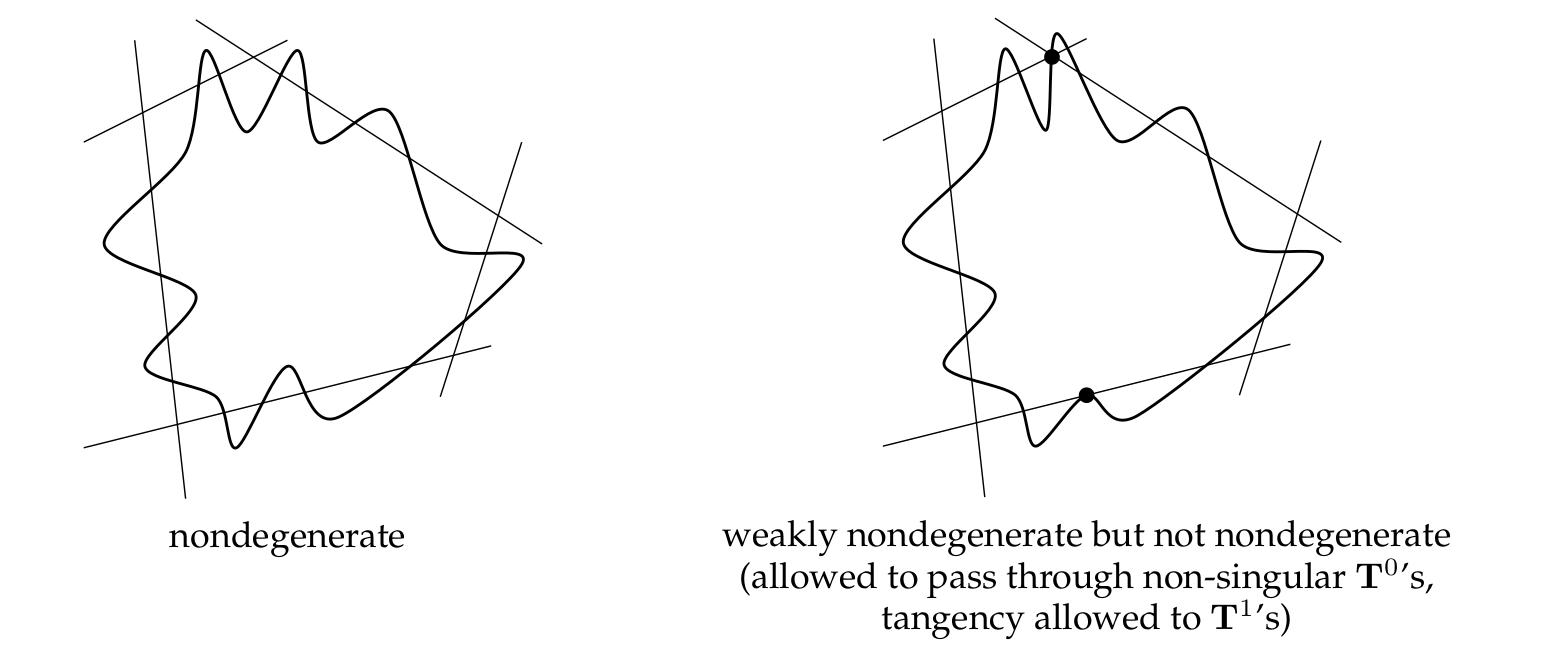
\includegraphics[width=\textwidth]{nondegeneracy}
\caption{The intersection properties of a curve with the toric divisor distinguishes nondegeneracy from weak nondegeneracy. Specifically for the curve to be nondegenerate, it must meet the toric divisor transversally and away from the codimension two $\Toric$-invariant divisors (Image credit \cite{WC_preface}).}
\end{figure}
\par
This condition on the nature of the intersection with the toric boundary is less intrinsic to the curve (for example, fixing a $\Gm{k}^2 \subset \P^2_k$ and a plane curve $C \subset \P^2_k$ we can always move the curve such that it intersects the three lines of the compliment of the torus transversally and does not pass through the intersection points of these three lines) and will often be inconsequential for results we would like to prove about such objects. Thus we define the weaker notion which ignores this intersection criterion.

\begin{defn}
We say that a Laurent polynomial $f \in k[x^{\pm 1}, y^{\pm 1}]$ is $\Delta$-\textit{toric} if $\Delta(f) \subset \Delta$ and $f$ defines a smooth curve $C_0 = U_f$ whose completion $C^\Delta_0 \embed \Toric_\Delta$ is smooth.
\end{defn}
\noindent
In the next section we will see how to reinterpret this condition purely in terms of properties of $f$, its Newton polygon, and the affine curve $U_f$.


\subsection{Baker's Theorem on the Genus for Toric Embeddings}

In this section, we discuss the classical result of Baker (1893) relating the genus of a smooth curve compactified in a toric surface to the enumerative properties of its associated convex lattice polygon.

\begin{thm}[Baker]
Let $f \in k[x^{\pm 1}, y^{\pm 1}]$ be a $\Delta$-nondegenerate Laurent polynomial. Then the toric completion $C_0^\Delta \embed \Toric_\Delta$ of $C_0 = U_f$ is a smooth Cartier divisor on $\Toric_\Delta$ and thus $C_0^\Delta$ is the unique smooth proper curve birational to $C_0$. Furthermore, the genus is computed via the number of interior lattice points of the Newton polygon, 
\[ g(C_0^\Delta) = |\Delta^\circ \cap \Z^2| \]
\end{thm}

\begin{proof}
Since $f$ is $\Delta$-nondegenerate, then $C_0^\Delta$ is an integral codimension one closed subscheme which does not intersect the singular locus of $\Toric_\Delta$ (in particular, if $x \in C_0^\Delta$ then $\stalk{\Toric_\Delta}{x}$ is a UFD) so $C_0^\Delta$ is Cartier. Since, by Lemma \ref{lemma_nondegeneracy}, the completion $C = C_0^\Delta$ is a smooth proper curve, its genus\footnote{If we assume $|\Delta^\circ \cap \Z^2| > 0$, then we do indeed have $H^0(C, \struct{C}) = k$ because the cokernel of $H^0(X, \struct{X}) \to H^0(C, \struct{C})$ is $H^1(X, \struct{X}(-D_C))$ which vanishes by the Batyrev-Borisov Vanishing theorem \cite[Thm. 9.2.7]{cox} because $\dim{\Delta} > 1$ and $D_C$ is ample. Regardless, we will find that $\dim_k H^0(C, \omega_C) = |\Delta^\circ \cap \Z^2|$ so $g(C) = |\Delta^\circ \cap \Z^2|$ in either case.} is $g(C) = \dim_k H^0(C, \Omega_{C/k})$ and $\Omega_{C/k} = \omega_{C}$ is its dualizing sheaf. Thus, we aim to compute $H^0(C, \Omega_C)$. Fixing notation, let $X = \Toric_\Delta$ and let $\iota : C \embed X$ be the inclusion. Choose a torus-invariant Cartier divisor $D_C$ linearly equivalent to the effective Cartier divisor $C$, in fact, we can explicitly write $D_C = C - \div{(f)}$ which is torus-invariant because it is supported on the toric divisor since $C|_{\Toric^n} = \div{(f)}|_{\Toric^n}$. We will now apply the adjunction exact sequence defined in Theorem \ref{adjunction},
\begin{center}
\begin{tikzcd}
0 \arrow[r] & \omega_X \arrow[r, "f"] & \omega_X(D_C) \arrow[r] & \iota_* \omega_C \arrow[r] & 0
\end{tikzcd}
\end{center}
Taking cohomology gives the following long exact sequence,
\begin{center}
\begin{tikzcd}
0 \arrow[r] & H^0(X, \omega_X) \arrow[r] & H^0(X, \struct{X}(D_C + K_X)) \arrow[r] & H^0(C, \omega_C) \arrow[r] & H^1(X, \omega_X)
\end{tikzcd}
\end{center} 
But $H^0(X, \omega_X) = H^0(X, \struct{X}(K_X)) = 0$ since the canonical divisor    has an empty corresponding polytope $P_{K_X} = \varnothing$. Furthermore, $H^1(X, \omega_X) = H^0(X, \struct{X}) = 0$ by Serre duality and Demazure vanishing. Therefore, the cohomology sequence gives an isomorphism,
\[ H^0(X, \struct{X}(D_C + K_X)) \xrightarrow{\sim} H^0(C, \omega_C) \]
In particular, the genus is,
\[ g(C) = \dim_k H^0(X, \struct{X}(D_C + K_X)) = | P_{D_C + K_X} \cap \Z^2 | \]
Thus, we need to compute $P_{D_C}$. Recall that under the embedding $\psi : \Toric_\Delta \embed \P^N_k$ the curve $C$ is the hyperplane section defined by the hyperplane,
\[ H_C = \sum_{(i, j) \in \Delta} a_{ij} X_{ij} \quad \text{ where } \quad f = \sum_{(i,j) \in \Delta} a_{ij} x^i y^j \]
Therefore, $\struct{X}(C) = \psi^* \struct{\P^N}(H_C) \cong \psi^* \struct{\P^N}(1)$ but recall that $\struct{X}(D_\Delta) = \psi^* \struct{\P^N}(1)$ so we find that $\struct{X}(C) \cong \struct{X}(D_\Delta)$. Therefore, $D_C \sim C \sim D_\Delta$ but both $D_C$ and $D_\Delta$ are torus-invariant so $P_{D_C} \cong_t \Delta$ (using that $P_{D_\Delta} = \Delta$). Decomposing,
\[ \Delta = \bigcap_{\substack{F \subset \Delta \\ \text{facet}}} H^+(n_F, - a_F) \]
we find,
\[ D_C \sim \sum_{\substack{F \subset \Delta \\ \text{facet}}} a_F D_F \]
Recall the canonical divisor is,
\[ K_X = - \sum_{\substack{F \subset \Delta \\ \text{facet}}} D_F \]
Thus,
\[ D_C + K_X \sim \sum_{\substack{F \subset \Delta \\ \text{facet}}} (a_F - 1) D_F \]
which implies that,
\[ P_{D_C + K_X} \cong_t \bigcap_{\substack{F \subset \Delta \\ \text{facet}}} H^+(n_F, 1 - a_F) = \Delta^{(1)} \]
since $\Delta$ is a lattice polygon. Therefore, we conclude,
\[ g(C) = | \Delta^{(1)} \cap \Z^2 | = | \Delta^\circ \cap \Z^2 | \]
\end{proof}

\begin{comment}

(RELATE THIS ABOVE FACT TO CANONICAL EMBEDDING)

\end{comment}

\begin{theorem} \label{adjunction}
Let $X$ be a normal projective Cohen-Macaulay variety, $\iota : C \embed X$ a prime divisor, and $D_C = C - \div{(f)}$ any linearly equivalent Weil divisor. Then there is an exact sequence,
\begin{center}
\begin{tikzcd}
0 \arrow[r] & \omega_X \arrow[r, "f"] & \omega_X(D_C) \arrow[r] & \iota_* \omega_C \arrow[r] & 0
\end{tikzcd}
\end{center}
\end{theorem}

\begin{rmk}
We will apply this theorem in the case when $D_C$ is chosen to be a $\Toric$-invariant Weil divisor but the proof does not depend on this fact.
\end{rmk}

\begin{proof}
The sheaf $\struct{X}(-D_C)$ is isomorphic to the sheaf of ideals defining $\iota : C \embed X$ giving an exact sequence,
\begin{center}
\begin{tikzcd}
0 \arrow[r] & \struct{X}(-D_C) \arrow[r, "f"] & \struct{X} \arrow[r] & \iota_* \struct{C} \arrow[r] & 0
\end{tikzcd}
\end{center}
Applying the functor $\shHom{\struct{X}}{-}{\omega_X}$ to the above short exact sequence gives a long exact sequence,
\begin{center}
\begin{tikzcd}
0 \arrow[r] & \shHom{\struct{X}}{\iota_* \struct{C}}{\omega_X} \arrow[r] \arrow[draw=none]{d}[name=Z, shape=coordinate]{} & \shHom{\struct{X}}{\struct{X}}{\omega_X} \arrow[r, "f"] & \shHom{\struct{X}}{\struct{X}(-D_C)}{\omega_X} 
\arrow[dll,
rounded corners, crossing over,
to path={ -- ([xshift=2ex]\tikztostart.east)
|- (Z) [near end]\tikztonodes
-| ([xshift=-2ex]\tikztotarget.west)
-- (\tikztotarget)}]
\\
& \shExt{1}{\struct{X}}{\iota_* \struct{C}}{\omega_X} \arrow[r] & \shExt{1}{\struct{X}}{\struct{X}}{\omega_X} \arrow[r] & \cdots
\end{tikzcd}
\end{center}
Since $\shHom{\struct{X}}{\struct{X}}{-}$ is the identity functor, $\shExt{1}{\struct{X}}{\struct{X}}{-} = 0$. Also, $\shHom{\struct{X}}{\iota_* \struct{C}}{\omega_X} = 0$ because $\iota_* \struct{C}$ is torsion but $\omega_X$ is torsion-free \cite[Ch. 1, Prop. 2.8]{grothendieck_duality}. Therefore, we find an exact sequence,
\begin{center}
\begin{tikzcd}
0 \arrow[r] & \omega_X \arrow[r, "f"] & \shHom{\struct{X}}{\struct{X}(-D_C)}{\omega_X} \arrow[r] & \shExt{1}{\struct{X}}{\iota_* \struct{C}}{\omega_X} \arrow[r] & 0
\end{tikzcd}
\end{center}
However, $X$ is Cohen-Macaulay (and projective) and $C$ is in codimension one so $\shExt{1}{\struct{X}}{\iota_* \struct{C}}{\omega_X}$ computes the dualizing sheaf $\iota_* \omega_C$ by \cite[Ch 1, Prop. 2.3]{grothendieck_duality}.
When $X$ is a normal projective variety, by Theorem \ref{canonical_reflexive}, the dualizing sheaf is reflexive with an associated canonical divisor Weil divisor $\omega_X = \struct{X}(K_X)$. Furthermore, by Theorem \ref{properties_of_reflexive_sheaves},
\[ \shHom{\struct{X}}{\struct{X}(-D_C)}{\omega_X} = \struct{X}(D_C + K_X) \]
Thus, we do get an exact sequence,
\begin{center}
\begin{tikzcd}
0 \arrow[r] & \struct{X}(K_X) \arrow[r, "f"] & \struct{X}(D_C + K_C) \arrow[r] & \iota_* \omega_C \arrow[r] & 0
\end{tikzcd}
\end{center}
viewing $f$ as a section of $\struct{X}(D_C)$, using that $D_C + \div{(f)} = C$ is effective, gives $\struct{X} \xrightarrow{f} \struct{X}(D_C)$. Then, tensoring by $- \otimes_{\struct{X}} \omega_X$ and using $\struct{X}(D) \otimes_{\struct{X}} \struct{X}(E) \to \struct{X}(D + E)$ via $f \otimes g \mapsto fg$ gives the above map.
\end{proof}

\noindent
The previous theorem shows that $\Delta$-nondegeneracy is sufficient for the closure of $U_f$ to embed smoothly. However, it is not necessary since the condition requires that the curve does not pass through the codimension-two toric components. We will use the following remark to weaken our nondegeneracy condition on $f$. First, we prove an extension of Baker's theorem which applies without the nondegeneracy condition.

\begin{thm} \label{baker_refinement}
For \textit{any} Laurent polynomial $f \in k[x^{\pm 1}, y^{\pm 1}]$ such that $U_f$ is a curve and $\Delta(f) = \Delta$,
\[ g(U_f) \le | \Delta^\circ \cap \Z^2 | \]
with equality exactly when the scheme theoretic image of $U_f \embed \Toric_\Delta$ is smooth. 
\end{thm}

\begin{proof}
See \cite[Section 2]{tim} and \cite[Section 2]{WC_zeta_functions}. Here, we will give a sketch of the proof. Let $V \subset \Delta$ be the vertices and $S = (\Delta \cap \Z^2) \setminus V$ the non vertex lattice points. Then, the parameter space of Laurent polynomials $f \in k[x^{\pm 1}, y^{\pm 1}]$ such that $\Delta(f) = \Delta$ is exactly $L = \A_k^{S} \times_k \Gm{k}^V$ with coordinates $x_{ij}$ for $(i,j) \in \Delta$, where we associate a $k$-rational point $(a_{ij}) \in \A_k^{S} \times_k \Gm{k}^V$ to the Laurent polynomial,
\[ f = \sum_{(i,j) \in \Delta} a_{ij} x^i y^j \]
Note that $\Delta(f) = \Delta$ since the coefficients $a_{ij}$ corresponding to vertices $(i,j) \in \Delta$ are nonzero.
Now, consider the closed subscheme,
\[ V \subset \Gm{k}^2 \times_k \A_k^{S} \times_k \Gm{k}^{V} = \Spec{k[x^{\pm 1}, y^{\pm 1}]} \times \Spec{k[(a_{ij})_{(i, j) \in S}, (a_{i,j}^{-1})_{(i,j) \in V}]} \]
defined by the vanishing,
\[ V = V\left( \sum_{(i,j) \in \Delta} a_{ij} x^i y^j \right) \]
Then the projection gives a family $\pi : V \to L$ of torus curves parameterized by the coefficients of their Laurent polynomials. Now, we complete $V$ under the open immersion $\Gm{k}^2 \times_k L \embed \Toric_\Delta \times_k L$ to get a closed immersion $\C \embed \Toric_\Delta \times_k L$ whose fiber over $f$ gives the $\Delta$-toric completion of $U_f$, 
\begin{center}
\begin{tikzcd}[row sep = huge]
V \arrow[r, hook] \arrow[drr] & \C \arrow[r, hook] \arrow[dr] & \Toric_\Delta \times_k L \arrow[d, "\pi"]
\\
& & L
\end{tikzcd}
\end{center}
By \cite[Section 2, Prop. 1]{WC_zeta_functions}, the locus of $L$ corresponding to $\Delta$-nondegenerate $f$ contains a Zariski dense open. Therefore, the general fiber $\mathcal{C}_{f_0}$ above $f_0 \in k[x^{\pm 1}, y^{\pm 1}]$ corresponds to $C_0^\Delta$, the completion of $C_0 = U_{f_0}$, which is smooth proper curve with genus and thus arithmetic genus,
\[ g_a(U_f^\Delta) = g(U_f^\Delta) = | \Delta^\circ \cap \Z^2 | \]
by the version of Baker's theorem proven above.
\bigskip\\
I claim the family $\C \to L$ is flat. First, the projection $X = \Toric_{\Delta} \times_k L \to L$ is flat meaning that $\stalk{L}{\pi(x)} \to \stalk{X}{x}$ makes $\stalk{X}{x}$ a flat $\stalk{L}{\pi(x)}$-module. The Laurent polynomial $f$ is a section of the line bundle $\struct{\Toric_\Delta}(D_\Delta) \boxtimes \struct{L}$ which is generated by the global sections $x^i y^j$ for $(i,j) \in V$ by Lemma \ref{polytope_div_ample}. Furthermore, coefficient functions $a_{ij} \in \Gamma(L, \struct{L})$ with $(i,j) \in V$ are non-vanishing. Since it suffices to check flatness on closed points, take any closed point $x \in \Toric_\Delta \times_k L$, then the germ $f \in \stalk{X}{x} / \m_{\pi{x}} \stalk{X}{x} = \stalk{X}{x}\otimes_{\stalk{L}{\pi(x)}} \kappa(\pi(x))$ is a zero divisor exactly when $f$ is the zero polynomial after evaluating the coefficients at $\pi(x) \in L$. However, all the $a_{ij}$ with $(i, j) \in V$ are non-vanishing on $L$ so $f \in \stalk{X}{x} / \m_{\pi{x}} \stalk{X}{x}$ is never the zero polynomial. Then applying \cite[\href{https://stacks.math.columbia.edu/tag/046Z}{Tag 046Z}]{stacks-project} we see that $\stalk{L}{\pi(x)} \to \stalk{X}{x}/(f)$ is flat and thus $\C \to L$ is flat.
\bigskip\\
Furthermore, $\C \embed \Toric_\Delta \times_k L\embed \P^n_k \times_k L$ is a closed subscheme so applying \cite[Thm. III.9.10]{har}, the arithmetic genus of the fibers is constant. Thus, for any $f \in k[x^{\pm 1}, y^{\pm 1}]$ such that $U_f$ is a smooth curve, then its toric completion $U_f^\Delta$ has arithmetic genus,
\[ g_a(U_f^\Delta) = g_a(C_0^\Delta) = | \Delta^\circ \cap \Z^2 | \]
We use Lemma \ref{genus_formulas} to conclude that,
\[ g(U_f) = g(U_f^\Delta) \le g_a(U_f^\Delta) = | \Delta^\circ \cap \Z^2 | \]
and an equality exactly when $U_f^\Delta$ is smooth. Furthermore, since $\C \to L$ is a proper flat family, by Zariski connectedness the fibers are connected so we see that \textit{any} $U_f^\Delta$ with $\Delta(f) = \Delta$ is connected (even when $U_f$ is not a curve, e.g. $U_f$ not connected).
\end{proof}

\begin{rmk}
We have shown that $U_f^\Delta$ is connected whenever $\Delta(f) = \Delta$ but the affine curve $U_f$ certainly may not be. For example, consider $f_1 = (x + y - 1)(x + y + 1)$ and $f_2 = x^2 + y^2 - 1$ then $\Delta(f_1) = \Delta(f_2) = 2 \Sigma$ where $\Sigma$ is the unit isosceles right triangle. However, 
\[ U_{f_1} = \Spec{k[x^{\pm 1}, y^{\pm 1}]/(f_1)} = \Spec{k[k[x^{\pm 1}, y^{\pm 1}]/(x + y - 1)} \times_k \Spec{k[k[x^{\pm 1}, y^{\pm 1}]/(x + y + 1)} \]
which is the union of two parallel lines in $\Gm{k}^2$ (which do not intersect in the torus) while,
\[ U_{f_2} = \Spec{k[x^{\pm 1}, y^{\pm 1}]/(f_2)} = \Spec{k[x^{\pm 1}, y^{\pm 1}]/(x^2 + y^2 - 1)} \]
is irreducible and thus connected. However, in the toric completion $U_{f_1}^\Delta$ (which lies in $\Toric_{2 \Sigma} = \P^2_k$), these two parallel lines do in fact intersect so both $U_{f_1}^\Delta$ and $U_{f_2}^\Delta$ are connected.
\end{rmk}


\begin{defn} \label{weakly_defn}
We say that $f \in k[x^{\pm 1}, y^{\pm 1}]$ is \textit{weakly} $\Delta$-\textit{nondegenerate} when the following hold,
\begin{enumerate}
\item $\Delta(f) \subset \Delta$
\item for each face $\tau \subset \Delta$ we have $\tau \cap \Delta(f) \neq \empty$
\item the affine curve $U_f$ is smooth with genus $g(U_f) = | \Delta^{(1)} \cap \Z^2 |$. 
\end{enumerate}
\end{defn}
\noindent
Weakly $\Delta$-nondegenerate Laurent polynomials $f \in k[x^{\pm 1}, y^{\pm 1}]$ do indeed define affine curves $U_f$ with an embedding $U_f \embed \Toric_\Delta$ such that the completion $C_0^\Delta$ is smooth and satisfies the numerical genus condition of Baker. However, such curves will not, in general, be Cartier divisors on $\Toric_\Delta$ since they may pass through the singular locus where $\Toric_\Sigma$ is not locally factorial. 

\begin{lemma}
Assuming parts (a) and (b) of Definition \ref{weakly_defn}, part (c) is equivalent to the condition that the scheme-theoretic image of $U_f \embed \Toric_\Delta$ is smooth. 
\end{lemma}

\begin{proof}
When $U_f^\Delta$ is smooth, $g(U_f^\Delta) = g_a(U_f^\Delta) = | \Delta^\circ \cap \Z^2|$. Conversely, we have that $\tilde{\Delta} = \Delta(f) \subset \Delta$ (from the definition that $f$ is weakly $\Delta$-nondegenerate) and we assume $g(U_f) = | \Delta^\circ \cap \Z^2 |$. From Baker's bound,
\[ g(U_f^\Delta) = g(U_f) \le |\tilde{\Delta}^\circ \cap \Z^2| \le |\tilde{\Delta}^\circ \cap \Z^2 | \] 
Thus, from the assumption these are equalities so,
\[ g(U_f^\Delta) = | \tilde{\Delta}^\circ \cap \Z^2 | \]
and thus $U_f^\Delta$ is smooth by the above result.
\end{proof}

\begin{comment}

\subsection{Combinatorial Gonality (WIP)}

\begin{defn}
Let $C$ be a curve over $k$. The \textit{gonality} $\gon{C}$ is defined to be the minimal degree of a non-constant morphism $C \to \P^1_k$. 
\end{defn}

\end{comment} 

\subsection{The Inverse Situation}

Up until now we have discussed the situation of specifying a curve by a fixed Laurent polynomial and attempting to describe the unique smooth complete curve in its birationality class via a toric completion. Here we consider the inverse problem: given a (smooth complete) curve $C$, we might ask when one can find a dense open set $U \subset C$ with a closed embedding $U \embed \Gm{k}^2$ such that the resultant Laurent polynomial describing the torus curve $U$ satisfies the nondegeneracy conditions we have discussed earlier. 

\begin{defn}
Given a convex lattice polygon $\Delta$, we say that a curve $C$ over $k$ is \textit{(weakly)} $\Delta$-\textit{nondegenerate} over $k$ if it is birational over $k$ to a curve $U \subset \Toric^2$ such that $U = V(f)$ for some (weakly) $\Delta$-nondegenerate Laurent polynomial $f \in k[x^{\pm 1}, y^{\pm 1}]$. In the case that $C$ is weakly $\Delta$-nondegenerate, we will alternatively say that $C$ is $\Delta$-toric to emphasize that $C$ embeds into the toric surface $\Toric_\Delta$. Furthermore, we say that $C$ is \textit{geometrically (weakly)} $\Delta$-\textit{nondegenerate} if $C \times_k \bar{k}$ is (weakly) $\Delta$-nondegenerate over $\bar{k}$.  
\end{defn}
\noindent\\
First we note that using the terms weakly $\Delta$-nondegenerate and $\Delta$-toric interchangeably will introduce no confusion because of the following result which shows that any curve which may be embedded in a toric surface is weakly nondegenerate.

\begin{prop}
Let $C \embed \Toric_\Delta$ be an embedding of a non-rational smooth curve into a toric surface. Then $C$ is weakly $\tilde{\Delta}_C$-nondegenerate where $\tilde{\Delta}_C = \Conv{P_C \cap \Z^2}$. 
\end{prop}

\begin{proof}
Since $C$ is nonrational, it cannot lie in the toric divisor $D_\Toric$ which is a union of toric varieties which are rational because every irreducible subvariety of the toric divisor is rational. Therefore it must intersect the torus, $C \cap \Toric^2 \neq \varnothing$ so $C \cap \Toric^2$ gives some curve $U_f \subset \Gm{k}^2$ defined by an irreducible Laurent polynomial $f \in k[x^{\pm 1}, y^{\pm 1}]$. Then the linearly equivalent divisor $D_C = C - \div{(f)}$ is torus-invariant since it is supported on $D_\Toric$ because $C |_{\Toric^2} = \div{(f)} |_{\Toric^2}$ on the torus. 
\bigskip\\
Now we consider the rational polytope $P_{D_C}$ of the torus-invariant Weil divisor $D_C$ (note $D_C$ may not be Cartier and $P_{D_C}$ may not be a lattice polytope). However, $D_C + \div{(f)} = C$ is effective so $f \in H^0(\Toric_\Delta, \struct{\Toric_\Delta}(D_C))$ which implies that $\Delta(f) \subset P_{D_C}$ because there is a decomposition,
\[ H^0(\Toric_\Delta, \struct{\Toric_\Delta}(D_C)) = \bigoplus_{(i,j) \in P_{D_C} \cap \Z^2} k \cdot x^i y^j \]
so the support of $f$ must be contained in $P_{D_C} \cap \Z^2$. Even better, this shows that,
\[ \Delta(f) \subset \Conv{P_{D_C} \cap \Z^2} = \tilde{\Delta}_C \subset P_{D_C} \]
Now, since $C$ is smooth, by our refinement of Baker's bound (Theorem \ref{baker_refinement}) we have,
\[ g(C) \le |\Delta(f)^{(1)} \cap \Z^2| \le |\tilde{\Delta}_C^{(1)} \cap \Z^2 | \]
As in the proof of Baker's theorem, we want to apply the exact sequence of Theorem \ref{adjunction},
\begin{center}
\begin{tikzcd}
0 \arrow[r] & \struct{X}(K_X) \arrow[r] & \struct{X}(D_C + K_X) \arrow[r] & \struct{C}(K_C) \arrow[r] & 0
\end{tikzcd}
\end{center}
which gives an isomorphism $H^0(X, \struct{X}(D_C + K_X)) \xrightarrow{\sim} H^0(C, \omega_C)$. 
\end{proof}

\begin{rmk}
Notice, in the proof of Theorem \ref{baker_refinement}, we use the fact (proven in \cite[Section 2, Prop. 1]{WC_zeta_functions}) that the generic Laurent polynomial $f \in k[x^{\pm 1}, y^{\pm 1}]$ with fixed Newton polygon $\Delta$ is $\Delta$-nondegenerate. However, we have shown that a very general curve cannot lie on any toric surface and thus cannot be $\Delta$-toric let alone $\Delta$-nondegenerate. How can these facts be consistent? It must be that under the equivalence relation,
\[ f \sim f' \iff U_f \birat U_{f'} \iff \Frac{k[x^{\pm 1},y^{\pm 1}]/(f)} \cong \Frac{k[x^{\pm 1},y^{\pm 1}] / (f')} \]
a general equation does not define a class corresponding to a general curve. In fact, the general Laurent polynomial $f \in k[x^{\pm 1}, y^{\pm 1}]$ with fixed $\Delta = \Delta(f)$ lies in the subspace of the moduli space corresponding to $\Delta$-nondegenerate curves.
\end{rmk}

Since the two notions are very similar, we naturally ask if weak and strong $\Delta$-regularity are equivalent properties. Restricting to a fixed lattice polygon $\Delta$, Castryck has provided a negative answer to this question by constructing a weakly $\Delta$-nondegenerate curve with no embedding into $\Toric_\Delta$ which intersects the toric divisor transversally. In particular, he showed the following.

\begin{prop} \label{example_weak_only}
There exists a lattice polygon $\Delta$ and a curve $C$ such that $C$ is weakly $\Delta$-nondegenerate but not $\Delta$-nondegenerate. Specifically, consider the Laurent polynomial,
\[ f = x^5 + y^2 + x^2 y^3 + 1 \in k[x^{\pm 1}, y^{\pm 1}] \]
and the lattice polygon $\Delta = \Conv{\{ (0,0), (5, 0), (2, 3), (0,3) \}}$.
\begin{figure}
\begin{center}
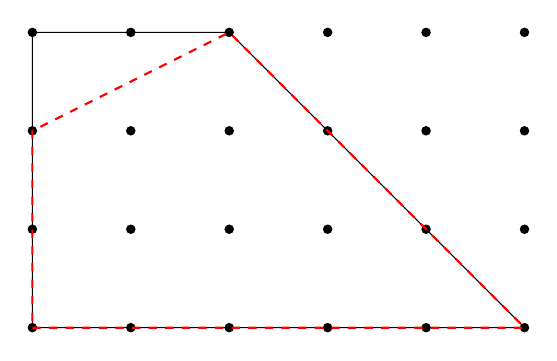
\begin{tikzpicture}

\foreach \x in {0,1,2,3,4,5}
   \foreach \y in {0,1,2,3} 
      \draw[fill] (5/4*\x,5/4*\y) circle (1.5pt) coordinate (m-\x-\y);

% using named coordinates
\draw (m-0-0) -- (m-5-0) -- (m-2-3) -- (m-0-3) -- cycle;
\draw[red, dashed, thick] (m-0-0) -- (m-5-0) -- (m-2-3) -- (m-0-2) -- cycle;
\end{tikzpicture}
\end{center}
\caption{The polygons $\Delta$ in black and $\Delta(f)$ in red for $f = x^5 + y^2 + x^2 y^3 + 1$ in example of Proposition \ref{example_weak_only}.}
\end{figure}
\end{prop}

\begin{proof}
See \cite[Lemma 4.4]{WC_linear_pencils}. The proof uses the theory of trigonal curves and the canonical embedding. Furthermore, for this particular choice of polygons, $\Delta^{(1)}$ and $\Delta$ have the same normal fan so we can identify the toric compactification of this curve with its canonical image. We can understand intuitively why this example works. The toric variety $\Toric_{\Delta}$ is a Hirzebruch surface and the curve $C_0^\Delta \embed \Toric_{\Delta}$ is tangent to the torus divisor at the component defined by the vertex $V = (0,3)$ in the polygon $\Delta$ showing that this curve is not $\Delta$-nondegenerate. Furthermore, the Hirzebruch surface has a single-parameter family of automorphism which translates the tangency point along the toric divisor. Thus no modification of $C_0$ can be $\Delta$-nondegenerate. Notice that $\Delta(f) \subsetneq \Delta$ and the normal fan of $\Delta(f)$ contains an additional ray. Therefore, $\Toric_{\Delta(f)}$ corresponds to the toric blowup of the tangency point which turns the tangency into a transverse intersection which explains why $f$ is $\Delta(f)$-nondegenerate although it is not $\Delta$-nondegenerate.
\end{proof}

\begin{figure}
\begin{center}
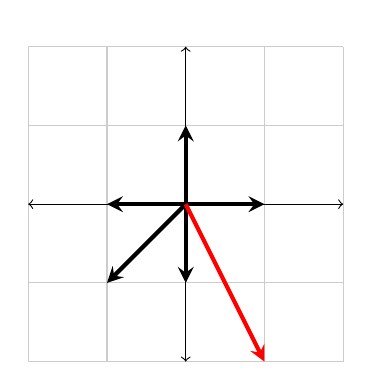
\begin{tikzpicture}
  \draw[thin,gray!40] (-2,-2) grid (2,2);
  \draw[<->] (-2,0)--(2,0) node[right]{};
  \draw[<->] (0,-2)--(0,2) node[above]{};
  \draw[line width=1.5pt,-stealth](0,0)--(-1,-1) node[anchor=south west]{$ $};
  \draw[line width=1.5pt,-stealth](0,0)--(-1,0) node[anchor=south west]{$ $};
  \draw[line width=1.5pt,-stealth](0,0)--(0,-1) node[anchor=south west]{$ $};
  \draw[line width=1.5pt,-stealth](0,0)--(0,1) node[anchor=north east]{$ $};
  \draw[line width=1.5pt,-stealth](0,0)--(1,0) node[anchor=south west]{$ $};
  \draw[line width=1.5pt,red,-stealth](0,0)--(1,-2) node[anchor=south west]{$ $};
\end{tikzpicture}
\end{center}
\caption{Rays of the normal fans of $\Delta$ (black) and $\Delta(f)$ (red). Notice that the normal fan of $\Delta(f)$ gives a toric blowup of the fan of $\Delta$.}
\end{figure}
\noindent
Notice that the curve Castryck constructs is actually nondegenerate (with respect to its own Newton polygon) and is only not nondegenerate for a specific choice of $\Delta$ for which it is weakly $\Delta$-nondegenerate. We suspect that there exist examples of curves which are $\Delta$-toric for some $\Delta$ but never $\Delta$-nondegenerate \textit{for any} $\Delta$. However, as of now, such examples remain elusive. Although we have shown that a very general curve cannot be $\Delta$-toric (let alone $\Delta$-nondegenerate) for any $\Delta$, low genus curves turn out to be well-behaved with respect to toric regularity. In particular, Castryck showed that all curves of genus $4$ or less admit a nondegenerate affine equation.


\begin{thm}[Cas17, Thm. 10]
Every curve $C / k$ of genus $g(C) \le 4$ is $\Delta$-nondegenerate for exactly one of a fixed finite list of lattice polygons.
\end{thm}


\begin{comment}


\subsection{Can We Give Example Never $\Delta$-nondegenerate (WIP)}


\subsection{Moduli Problem for Nondegenerate Curves (WIP)}


\subsection{Curves in Hirzebruch Surfaces (WIP)}

\end{comment}